\subsection{Kitöltés}

%47
\begin{frame}
  A kitöltések mindig átlátszók, csak a szélességük állítható:
  \begin{itemize}
    \item 1-4 érték megadásával, pl.\\
    \texttt{padding: 10px 20px 30px 40px;}\\
    (Fent, jobbra, lent, balra; további esetek mint \texttt{border-style}-nál.)
    \item Oldalakra vonatkozó tulajdonságokkal:\\
      \texttt{padding-*}, ahol \texttt{*} helyén állhat 
      \texttt{top}, \texttt{right}, \texttt{bottom}, \texttt{left}.
  \end{itemize}
\end{frame}

%48
\begin{frame}
  A kitöltés szélessége lehet:
  \begin{itemize}
    \item \texttt{inherit}: a befoglaló, szülő elem beállításait örökli
    \item CSS mértékegységgel (pl. \texttt{px}, \texttt{cm}) adott
    \item \texttt{\%}: a szülő elem méretének százaléka
  \end{itemize}
  \vfill
  Negatív értékek \kiemel{nem} használhatók.
\end{frame}

%49
\begin{frame}
  \begin{columns}[c]
    \column{0.25\textwidth}
      Próbálja meg elkészíteni az ábrának megfelelően a dobozokat!
    \column{0.7\textwidth}
      \begin{center}
        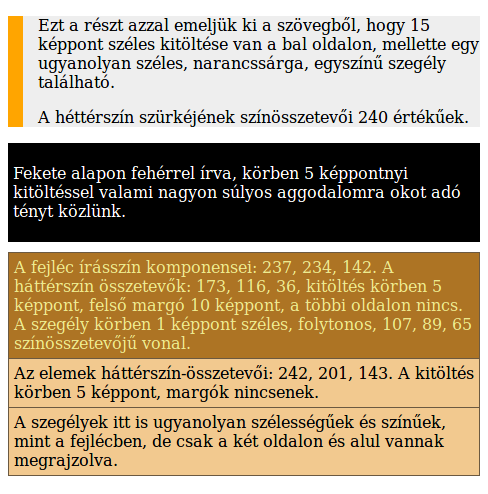
\includegraphics[scale=0.35]{dobozok.png}\\
        \textattachfile{dobozok.html}{dobozok.html}
      \end{center}
  \end{columns} 
\end{frame}
